\chapter{Rotman}
The big idea: algebraic topology assigns discrete algebraic invariants to
topological spaces and continuous maps. Book for this section: Joseph Rotman's
\emph{A First Course in Algebraic Topology}

\section{A sketch of the Brouwer Fixed Point Theorem}
\begin{problem}[R 0.1]
  Every continuous function $f : D^1 \to D^1$ has a fixed point.
\end{problem}
\begin{solution}
  We'll prove this without the techniques of analysis, so as to make the
  connection to the general argument slightly more obvious. Let $f(-1) = a$ and
  $f(1) = b$.
  \begin{enumerate}[label=(\arabic*)]
    \item Suppose $a = -1$ or $b = 1$, then we're done.
    \item Else, $a > -1$ and $b < 1$. Consider the graph of $f$:
      \[
        G = \set{\pn{x, f(x)} \MID x \in D^1}
      \]
      since $f$ is continuous and $D^1$ is connected, $G$ is connected as well.
      Let
      \[
        A = \set{\pn{x, f(x)} \MID f(x) > x} \qquad \text{and} \qquad B =
        \set{\pn{x, f(x)} \MID f(x) < x}.
      \]
      \begin{figure}[H]
        \centering
        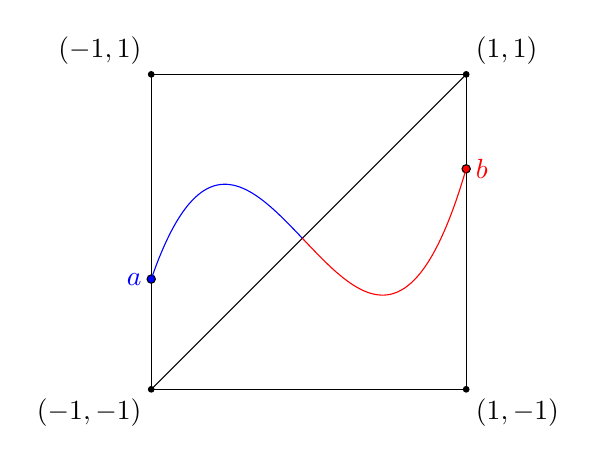
\begin{tikzpicture}[scale=2]
          \path
          coordinate (1) at (-1,-1)
          coordinate (2) at (-1,1)
          coordinate (3) at (1,1)
          coordinate (4) at (1,-1)
          coordinate (a) at (-1,-.3)
          coordinate (b) at (1, .4);

          \foreach \v in {1,2,3,4}{
            \draw[fill=black] (\v) circle (0.5pt);
          }

          \node[below left] (11) at (1) {$(-1,-1)$};
          \node[above left] (21) at (2) {$(-1,1)$};
          \node[above right] (31) at (3) {$(1,1)$};
          \node[below right] (41) at (4) {$(1,-1)$};

          \draw (1) -- (2) -- (3) -- (4) -- (1);
          \draw (1) -- (3);

          \draw[fill=blue] (a) circle (0.75pt);
          \draw[fill=red] (b) circle (0.75pt);
          \node[left] (ap) at (a) {$\color{blue}a$};
          \node[right] (bp) at (b) {$\color{red}b$};

          % \draw[domain=-1:1,smooth,variable=\x,blue] plot ({\x},{(-24 - 101*\x + 27*\x^2 + 122*\x^3)/60});
          \draw[domain=-1:-0.0405889,smooth,variable=\x,blue] plot ({\x},{\x*(\x*(1.4*\x + 0.133333) - 1.05) - 0.0833333});
          \draw[domain=-0.0405889:1,smooth,variable=\x,red] plot ({\x},{\x*(\x*(1.4*\x + 0.133333) - 1.05) - 0.0833333});

        \end{tikzpicture}
        \caption{$G$}
        \label{fig:brouwer-1}
      \end{figure}
      And let $\Delta = \set{\pn{x,x} \MID x \in [0,1]}$. Note $a \in A$, and $b
      \in B$, so $A \neq \varnothing \neq B$.

      Suppose $G \cap \Delta = \varnothing$. Then $G = A \sqcup B$. Note $A,B$
      are open in $G$, hence $G$ is not connected, a contradiction.
  \end{enumerate}
\end{solution}

\begin{definition}[retract]
  A subspace $X$ of a topological space $Y$ is a \emph{retract} of $Y$ if there
  is a continuous map $r : Y \to Y$ with $r(x) = x$ for all $x \in X$. Such a
  map is called a \emph{retraction}.
\end{definition}

% \begin{problem}[R 0.2]
%   If $n \geq 0$, then $S^n$ is not a retract of $D^{n+1}$
% \end{problem}
% \begin{solution}

% \end{solution}

\begin{problem}

\end{problem}

%%% Local Variables:
%%% TeX-master: "../main"
%%% End: